Let $\S$ be a totally ordered set with a binary relation $<$.
For any $x,y \in \S$, we can define the less-than and the equality functions as follows.
\begin{align*}
  \LT_\S(x,y) = 
  \begin{cases}
    1, & \text{if } x < y; \\
    0, & \text{if } x \ge y, \\
  \end{cases}
  \qquad
  \EQ_\S(x,y) = 
  \begin{cases}
    1, & \text{if } x = y; \\
    0, & \text{if } x \neq y. \\
  \end{cases}
\end{align*}
If $\S$ is a complete set of representatives of a finite field $\F_\fieldcard$, then the equality function can be easily realized using the principal character of $\F_\fieldcard$, namely $\EQ_\S(x,y) = 1 - \princhar_\fieldcard(x-y)$.
Since this function is independent of the choice of $\S$, we can write
\begin{align*}
  \EQ_{\F_{\fieldcard}}(x,y) = 1 - \princhar_\fieldcard(x-y).
\end{align*}
The less-than function can be interpolated using Lemma~\ref{lem:interpolation} and the following truth table
\begin{align*}
  \begin{array}{c|ccccc}
    < & a_0 & a_1 & a_2 & \cdots & a_{\fieldcard-1} \\
    \hline
    a_0 & 0 & 1 & 1 & \cdots & 1 \\
    a_1 & 0 & 0 & 1 & \cdots & 1 \\
    a_2 & 0 & 0 & 0 & \cdots & 1 \\
    \vdots & \vdots & \vdots & \vdots & \ddots & \vdots \\
    a_{\fieldcard-1} & 0 & 0 & 0 & \cdots & 0 \\
  \end{array}
\end{align*}
where $a_i \in \S$ for any $i \in [0,\fieldcard-1]$ and $a_i < a_j$ if $i < j$.
In particular,
\begin{align}\label{eq:less_than_function}
  \LT_\S(x,y) &= \sum_{a,b \in \S} \LT_\S(a,b) (1-\princhar_\fieldcard(x - a)) (1-\princhar_\fieldcard(y - b)) \nonumber\\
  &= \sum_{a \in \S} (1-\princhar_\fieldcard(x - a)) \sum_{b \in \S} \LT_\S(a,b)  (1-\princhar_\fieldcard(y - b)) \nonumber\\
  &= \sum_{a \in \S} (1-\princhar_\fieldcard(x - a)) \sum_{b \in \S, a < b} (1-\princhar_\fieldcard(y - b)).
\end{align}
In contrast to equality, this function depends on the choice of $\S$.
Nevertheless, we can fix a certain $\S$ as the default compelete set of representatives of $\F_{\fieldcard}$ and denote $\LT_\S(x,y)$ as $\LT_{\F_\fieldcard}(x,y)$.

The homomorphic circuit for $\LT_{\F_\fieldcard}(x,y)$ is presented in Algorithm~\ref{alg:basic_less_than_circuit}.
Unlike the prior works (\todo{cite}) that evaluate this circuit as a multivariate polynomial, we exploit its representation in~(\ref{eq:less_than_function}) to parallelize computations in the SIMD manner. 
\begin{algorithm}[t]
  \KwIn{
  $\ct_x$ -- a ciphertext encrypting $x \in \F_\fieldcard$ in the first SIMD slot and $0$ in other slots,
  $\ct_y$ -- a ciphertext encrypting $y \in \F_\fieldcard$ in the first SIMD slot and $0$ in other slots,
  $\S = \{a_0,a_1,\dots,a_{\fieldcard-1}\}$ -- a complete set of representatives of $\F_\fieldcard$.
  }
  \KwOut{$\ct$ -- a ciphertext encrypting $1$ in the first SIMD slot if $x < y$, otherwise $0$. Other slots contain $0$.}
  $\ct_1 \leftarrow \Replicate(\ct_x, \fieldcard - 1)$//\todo{Define replicate}\\
  $\ct_2 \leftarrow \Replicate(\ct_y, \fieldcard - 1)$\\
  $\pt_1 \leftarrow \pt(a_0, a_1, \dots, a_{\fieldcard-2})$//\todo{define this operation}\\
  $\pt_2 \leftarrow \pt(a_1, a_2, \dots, a_{\fieldcard-1})$\\
  $\ct_1 \leftarrow \ct_1 - \pt_1$//\todo{define operations between ciphertexts and plaintexts}\\
  $\ct_2 \leftarrow \ct_2 - \pt_2$\\
  $\ct_1 \leftarrow \ct_1^{\fieldcard-1}$//$\princhar_\fieldcard(x-a)$, \todo{define this operation}\\
  $\ct_2 \leftarrow \ct_2^{\fieldcard-1}$//$\princhar_\fieldcard(y-b)$\\
  $\ct_1 \leftarrow 1 - \ct_1$// define operations between constants and ciphertexts\\
  $\ct_2 \leftarrow 1 - \ct_2$\\
  $k \leftarrow 1$// compute all running sums $\sum_{b \in \S, a < b} (1-\princhar_\fieldcard(x - b))$ \\
  \While{$k < \fieldcard-1$}{
    $\ct_{tmp} \leftarrow \Shift(\ct_2, k)$//\todo{define shift}\\
    $\ct_2 \leftarrow \ct_2 + \ct_{tmp}$\\
    $k \leftarrow 2k$\\
  }
  $\ct \leftarrow \ct_1 \cdot \ct_2$\\
  $k \leftarrow 1$\\
  \While{$k < \fieldcard-1$}{
    $\ct_{tmp} \leftarrow \Shift(\ct, k)$\\
    $\ct \leftarrow \ct + \ct_{tmp}$\\
    $k \leftarrow 2k$\\
  }
  $\ct \leftarrow \Select(\ct, \{1\})$//\todo{define select}\\
  \textbf{Return} $\ct$.
  \caption{Homomorphic circuit of $\LT_{\F_\fieldcard}$.}\label{alg:basic_less_than_circuit}
\end{algorithm}
\todo{Make a separate algorithm for running sums (while circuit above)}
\todo{Write down the complexity of Algorithm~\ref{alg:basic_less_than_circuit}, compare with prior works}

\subsection{Lexicographic order}
  Let $\vx=(x_0,x_1,\ldots,x_{\ell-1})$ and $\vy=(y_0,y_1,\ldots,y_{\ell-1}) \in \F_\fieldcard^\ell$ for the lexicographical order $<$ defined by the choice of $\S$:
  \begin{align*}
    \vx < \vy \Leftrightarrow \exists i\in[0,\ell-1] \text{ such that } x_i < y_i \text{ and } \forall j > i ~~ x_j = y_j\,.
  \end{align*}
  This order induces a function $\LT_{\F_\fieldcard}(\vx, \vy)$ that returns $1$ if $\vx < \vy$ and $0$ otherwise. 
  As done in~\cite{TLWRK20}, we can employ $\EQ_{\F_\fieldcard}$ and $\LT_{\F_\fieldcard}$ to compute $\LT_{\F_\fieldcard}(\vx, \vy)$ as follows
  \begin{align*}
    \LT_{\F_\fieldcard}(\vx, \vy) = \sum_{i=0}^{\ell-2} \LT_{\F_\fieldcard}(x_{i}, y_{i}) \prod_{j=i+1}^{\ell-1} \EQ_{\F_\fieldcard}(x_{j}, y_{j}) + \LT_{\F_\fieldcard}(x_{\ell-1}, y_{\ell-1}).
  \end{align*}
  Notice that the multiplicative depth of this function solely depends on the products of the equality functions.
  In fact, these products compare subvectors $\vx_i = (x_i, x_{i+1},\dots,x_{\ell-1})$ and $\vy_i = (y_i, y_{i+1},\dots,y_{\ell-1})$ for $i \in [1,\ell-1]$.
  Thus, we can rewrite $\LT_{\F_\fieldcard}$ as
  \begin{align}\label{eq:general_lex_order}
    \LT_{\F_\fieldcard}(\vx, \vy) = \sum_{i=0}^{\ell-2} \LT_{\F_\fieldcard}(x_{i}, y_{i}) \EQ_{\F_\fieldcard}(\vx_{i+1}, \vy_{i+1}) + \LT_{\F_\fieldcard}(x_{\ell-1}, y_{\ell-1})
  \end{align}
  with the equality function $\EQ_{\F_\fieldcard}(\vx_{i+1}, \vy_{i+1})$ that returns $1$ if $\vx_{i+1} = \vy_{i+1}$ and $0$ otherwise.
  As shown in~\todo{cite our work}, this function can be realized by a constant-depth circuit in the following way.
  \begin{align}\label{eq:rand_eq_circuit}
    \EQ_{\F_\fieldcard, e}(\vx_{i+1},\vy_{i+1}) = 1 - \princhar_{\fieldcard^e}\left(\sum_{j=i+1}^{\ell-1} r_j (x_j - y_j)\right)
  \end{align}
  where $r_j$ are uniformly random elements from $\F_{\fieldcard^e}$.
  This circuit is false-biased with error probability $\fieldcard^{-e}$.
  We can compute all $\EQ_{\F_\fieldcard, e}(\vx_{i+1},\vy_{i+1})$ using the same number of multiplications as for the single equality using Algorithm~\ref{alg:vector_equalities_circuit}.\todo{What is the complexity?}
  \begin{algorithm}[t]
    \KwIn{
    $\ct_\vx$ -- a ciphertext encrypting $\vx \in \F^\ell_\fieldcard$,
    $\ct_\vy$ -- a ciphertext encrypting $\vy \in \F^\ell_\fieldcard$.
    }
    \KwOut{$\ct$ -- a ciphertext containing the output of $\EQ_{\F_\fieldcard, e}(\vx_{i+1},\vy_{i+1})$ in the $i$th SIMD slot}
    $\ct_1 \leftarrow \Shift(\ct_\vx, 1)$ // removes the value $x_0$ and shifts $\vx$ to the left\\
    $\ct_2 \leftarrow \Shift(\ct_\vy, 1)$ // removes the value $y_0$ and shifts $\vy$ to the left\\
    $\ct \leftarrow \Sub(\ct_1, \ct_2)$ // $(x_i - y_i), i \in [1,\ell-1]$\\
    $r_0,r_1,\dots,r_{\ell-1} \leftarrow \udist(\F_{\fieldcard^e})$ //\todo{define uniform distribution}\\ 
    $\pt_r \leftarrow \pt(r_0,r_1,\dots,r_{\ell-1})$\\
    $\ct \leftarrow \ct \cdot \pt_r$ // $r_i(x_i - y_i), i \in [1,\ell-1]$\\
    $k \leftarrow 1$// $\sum_{j=i}^{\ell-1} r_i(x_i - y_i), i \in [1,\ell-1]$\\
    \While{$k < \ell-1$}{
      $\ct_{tmp} \leftarrow \Shift(\ct, k)$\\
      $\ct \leftarrow \ct + \ct_{tmp}$\\
      $k \leftarrow 2k$\\
    }
    $\ct \leftarrow \Power(\ct, \fieldcard^e-1)$ //$\princhar_{\fieldcard^e}\left(\sum_{j=i}^{\ell-1} r_i(x_i - y_i)\right), i \in [1,\ell-1]$ \\
    $\ct \leftarrow 1 - \ct$\\
    \textbf{Return} $\ct$.
    \caption{Homomorphic circuit computing $\EQ_{\F_\fieldcard, e}(\vx_{i+1},\vy_{i+1})$ in parallel.}\label{alg:vector_equalities_circuit}
  \end{algorithm}
  
  Let us go back to the lexicographic order in equation~(\ref{eq:general_lex_order}).
  Assume that we have a ciphertext $\ct_{\LT}$ containing $\LT_{\F_\fieldcard}(x_i, y_i)$ in the $i$th slot (\todo{elaborate on that}) and the output $\ct_{\EQ}$ of Algorithm~\ref{alg:vector_equalities_circuit}.
  We set the $\ell-1$ slot of $\ct_{\EQ}$ to $1$ and multiply it by $\ct_{\LT}$.
  The resulting ciphertext contains all the products $\LT_{\F_\fieldcard}(x_{i}, y_{i}) \EQ_{\F_\fieldcard}(\vx_{i+1}, \vy_{i+1})$ for any $i \in [0,\ell-2]$ and $\LT_{\F_\fieldcard}(x_{\ell-1}, y_{\ell-1})$, which can be summed in the same way as in the while circuit of Algorithm~\ref{alg:vector_equalities_circuit}.
  As a result, we obtain a ciphertext with the output of $\LT_{\F_\fieldcard}(\vx, \vy)$ in the first SIMD slot.

  \subsubsection{Comparing large integers.}
  Since any integer $z$ can be represented in base $\fieldcard$ as $z = \sum_{i=0}^{\ell-1} z_i q^i$, we can encode $z$ into SIMD slots as a vector $(z_0,z_1,\dots,z_{\ell-1}) \in \F_{\fieldcard}^\ell$.
  As shown above, we can compare such vectors using the lexicographic order function in~(\ref{eq:general_lex_order}) and thus compare integers larger than $\fieldcard$.

  \todo{Incorporate the following into the complexity analysis.} 
  We can obtain ciphertexts encrypting $(x,x,\ldots, x)$ and $(y,y,\ldots, y)$ with $2\log_2(q-1)\texttt{Rot}$ and $2\log_2(q-1)\texttt{Add}$. 

  From there we can obtain encryptions of $(x,x-1,\ldots, x-q-2)$ and $(y-1,y-2,\ldots, y-q-1)$ with $2\texttt{Add}$. We can apply $f$ to these vectors in parallel with a depth of $\log (p-1) + \log d$ for a cost of $2(\log (p-1) + wt(p-1) + d - 2) \texttt{Mult}$. This can be minimized by choosing $p = 2^d + 1$ for some $d$.

  With $2$ more $\texttt{Sub}$ we obtain encryptions of $(1-f(x), 1-f(x-1), \ldots, 1-f(x-q-2))$ and $(1-f(y-1), 1-f(y-2), \ldots, 1-f(y-q-1))$. From there we can get an encryption of the different partial sums in $\log_2(q-1)\texttt{Rot}$, $\log_2(q-1)\texttt{Select}$ and $\log_2(q-1)\texttt{Add}$. The algorithm works as follow:

  \begin{center}
    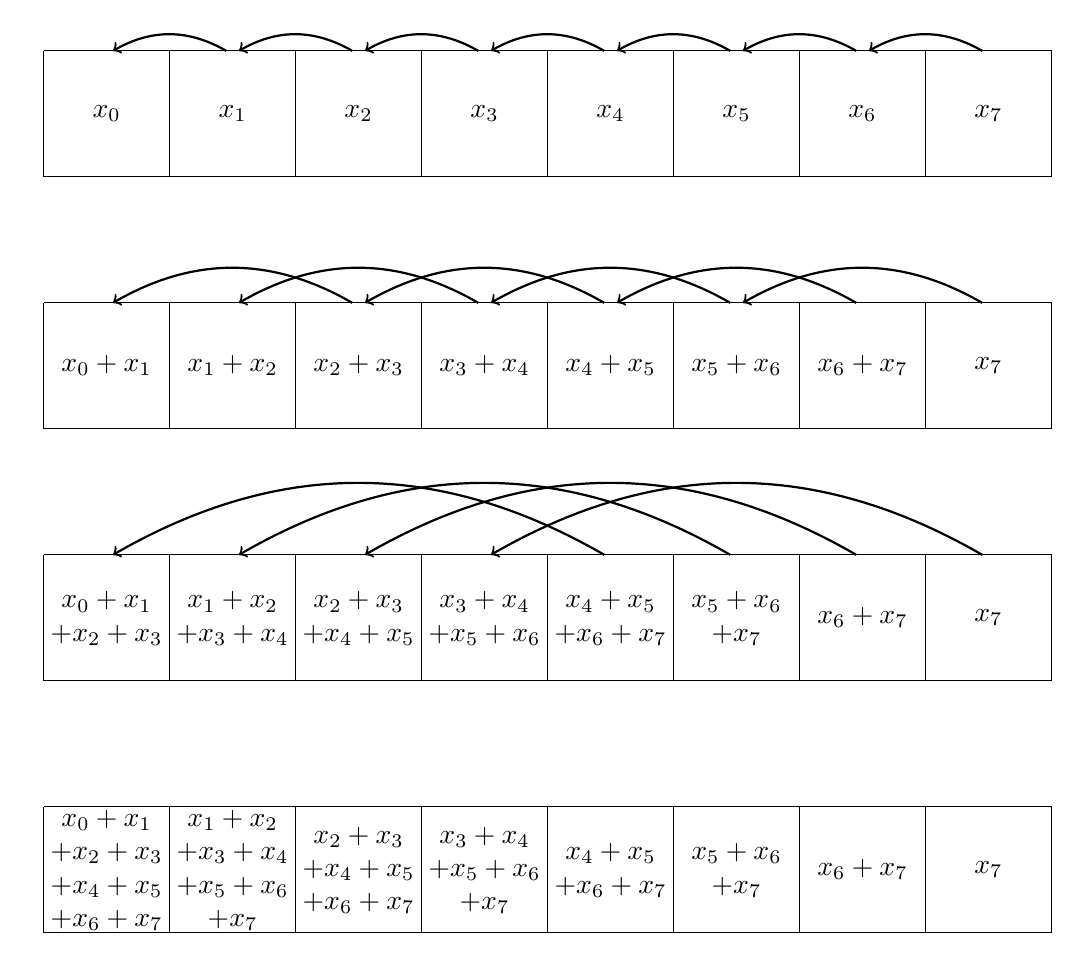
\begin{tikzpicture}[scale=0.8]
      \newcommand\y{-4};
      
      \draw (0,2) -- (16,2);
      \draw (0,0) -- (16,0);    
      \foreach \x in {0,...,8}{
        \draw (2*\x,0) -- (2*\x,2);
      }
      \foreach \x in {0,...,7}{
        \node at (2*\x+1,1) {$x_\x$};
      }

      \draw (0,2+\y) -- (16,2+\y);
      \draw (0,\y) -- (16,\y);    
      \foreach \x in {0,...,8}{
        \draw (2*\x,0+\y) -- (2*\x,2+\y);
      }

      \node at (1,1+\y) {$x_0 + x_1$};
      \node at (3,1+\y) {$x_1 + x_2$};
      \node at (5,1+\y) {$x_2 + x_3$};
      \node at (7,1+\y) {$x_3 + x_4$};
      \node at (9,1+\y) {$x_4 + x_5$};
      \node at (11,1+\y) {$x_5 + x_6$};
      \node at (13,1+\y) {$x_6 + x_7$};
      \node at (15,1+\y) {$x_7$};

      %%%%%%%%%%%%%%%%%%%%%%%%%%%%%%%%%%%%
      
      \draw (0,2+2*\y) -- (16,2+2*\y);
      \draw (0,0+2*\y) -- (16,0+2*\y);    
      \foreach \x in {0,...,8}{
        \draw (2*\x,0+2*\y) -- (2*\x,2+2*\y);
      }

      \node at (1,1+2*\y) {$\begin{array}{c}
          x_0 + x_1  \\
          + x_2 + x_3
        \end{array}$};
      \node at (3,1+2*\y) {$\begin{array}{c}
          x_1 + x_2  \\
          + x_3 + x_4
        \end{array}$};
      \node at (5,1+2*\y) {$\begin{array}{c}
          x_2 + x_3  \\
          + x_4 + x_5
        \end{array}$};
      \node at (7,1+2*\y) {$\begin{array}{c}
          x_3 + x_4  \\
          + x_5 + x_6
        \end{array}$};
      \node at (9,1+2*\y) {$\begin{array}{c}
          x_4 + x_5  \\
          +x_6 + x_7
        \end{array}$};
      \node at (11,1+2*\y) {$\begin{array}{c}
          x_5 + x_6  \\
          + x_7
        \end{array}$};
      \node at (13,1+2*\y) {$x_6 + x_7$};
      \node at (15,1+2*\y) {$x_7$};

      %%%%%%%%%%%%%%%%%%%%%%%%%%%%%%%%%%%%%%%%%%
      
      \draw (0,2+3*\y) -- (16,2+3*\y);
      \draw (0,0+3*\y) -- (16,0+3*\y);    
      \foreach \x in {0,...,8}{
        \draw (2*\x,0+3*\y) -- (2*\x,2+3*\y);
      }

      \node at (1,1+3*\y) {$\begin{array}{c}
          x_0 + x_1  \\
                              + x_2 + x_3 \\
                              + x_4 + x_5 \\
                              + x_6 + x_7
        \end{array}$};
      \node at (3,1+3*\y) {$\begin{array}{c}
          x_1 + x_2  \\
                              + x_3 + x_4 \\
                              + x_5 + x_6 \\
                              + x_7 \\
        \end{array}$};
      \node at (5,1+3*\y) {$\begin{array}{c}
          x_2 + x_3  \\
                              + x_4 + x_5 \\
                              + x_6 + x_7
        \end{array}$};
      \node at (7,1+3*\y) {$\begin{array}{c}
          x_3 + x_4  \\
                              + x_5 + x_6 \\
                              +x_7
        \end{array}$};
      \node at (9,1+3*\y) {$\begin{array}{c}
          x_4 + x_5  \\
          +x_6 + x_7
        \end{array}$};
      \node at (11,1+3*\y) {$\begin{array}{c}
          x_5 + x_6  \\
          + x_7
        \end{array}$};
      \node at (13,1+3*\y) {$x_6 + x_7$};
      \node at (15,1+3*\y) {$x_7$};

      \foreach \x in {2,...,8}
      \draw[->,thick = 2pt] (2*\x-0.1-1,2) to[bend right] (2*\x-3+0.1,2);

      \foreach \x in {3,...,8}
      \draw[->,thick = 2pt] (2*\x-0.1-1,2+\y) to[bend right] (2*\x-5+0.1,2+\y);

      \foreach \x in {5,...,8}
      \draw[->,thick = 2pt] (2*\x-0.1-1,2+2*\y) to[bend right] (2*\x-9+0.1,2+2*\y);

  \end{tikzpicture}
  \end{center}

  From there we just have to compute the scalar product of the two vectors with $1\texttt{Mult} + \log_2(q-1)\texttt{Rot} + \log_2(q-1)\texttt{Add}$. \newline

  So overall we can compute $<$ over $\mathbb{F}_q$ for $q = p^d$ in:

  \begin{itemize}
  \item $4\log_2 (q-1) \texttt{Rot}$
  \item $(4\log_2 (q-1) + 4) \texttt{Add}$
  \item $(2(\log (p-1) + wt(p-1) + d - 2) + 1) \texttt{Mult}$
  \item $(\log_2 (q-1) + 1) \texttt{Select}$
  \end{itemize}


%%% Local Variables:
%%% mode: latex
%%% TeX-master: "main"
%%% End:
